% answers.tex —— 2010 年·普通高等学校招生考试·浙江卷·文科 · 参考答案与详细解析片段
% 由 tools/generate_projects.py 依来源总账自 2010/2010_数学真题_浙江文_试题.md + 2010/2010_数学真题_浙江文_解析正文.md + 2010/2010_数学真题_浙江文_答案要点.md 生成，勿手改（改源 MD 后重跑）
\begin{gktip}
固定候选 PDF 仅含题面，无答案页；以下解析与结论均由本库独立推导（非官方答案），并按 600 dpi 原页复核题面。原页未印分值，不补。
\end{gktip}

\begin{answer}
\gksolhead{1}{}

\textbf{题目}：

设 $P=\{x\mid x<1\}$，$Q=\{x\mid x^2<4\}$，则 $P\cap Q=$（　）

（A）$\{x\mid -1<x<2\}$

（B）$\{x\mid -3<x<-1\}$

（C）$\{x\mid 1<x<4\}$

（D）$\{x\mid -2<x<1\}$

\Needspace{4\baselineskip}
\textbf{解析}
\Needspace{5\baselineskip}
$Q=\{x\mid x^2<4\}=\{x\mid -2<x<2\}$，$P=\{x\mid x<1\}$。两区间求交：
\nopagebreak[4]
\[P\cap Q=\{x\mid -2<x<2\}\cap\{x\mid x<1\}=\{x\mid -2<x<1\}.\]
故选 D。

\gkanswer{答案：D。}

\end{answer}
\begin{answer}
\gksolhead{2}{}

\textbf{题目}：

已知函数 $f(x)=\log_2(x+1)$，若 $f(\alpha)=1$，则 $\alpha=$（　）

（A）$0$

（B）$1$

（C）$2$

（D）$3$

\Needspace{4\baselineskip}
\textbf{解析}
\Needspace{5\baselineskip}
由对数定义域 $\alpha+1>0$ 且
\nopagebreak[4]
\[\log_2(\alpha+1)=1\iff\alpha+1=2^1=2,\]
故 $\alpha=1$。
故选 B。

\gkanswer{答案：B。}

\end{answer}
\begin{answer}
\gksolhead{3}{}

\textbf{题目}：

设 $\mathrm i$ 为虚数单位，则 $\dfrac{5-\mathrm i}{1+\mathrm i}=$（　）

（A）$-2-3\mathrm i$

（B）$-2+3\mathrm i$

（C）$2-3\mathrm i$

（D）$2+3\mathrm i$

\Needspace{4\baselineskip}
\textbf{解析}
\Needspace{5\baselineskip}
分子分母同乘 $1-\mathrm i$：
\nopagebreak[4]
\[\frac{5-\mathrm i}{1+\mathrm i}
=\frac{(5-\mathrm i)(1-\mathrm i)}{(1+\mathrm i)(1-\mathrm i)}
=\frac{5-5\mathrm i-\mathrm i+\mathrm i^2}{1-\mathrm i^2}
=\frac{4-6\mathrm i}{2}=2-3\mathrm i.\]
故选 C。

\gkanswer{答案：C。}

\end{answer}
\begin{answer}
\gksolhead{4}{}

\textbf{题目}：

某程序框图如图所示，若输出的 $S=57$，则判断框内为（　）

（A）$k>4$?

（B）$k>5$?

（C）$k>6$?

（D）$k>7$?
\nopagebreak[4]
\begin{center}% 2010 年浙江卷文科第 4 题：程序框图（判断框内容待填）。
% 来源 PDF：普通高考/2010/2010浙江文.pdf，SHA-256 a73e22ea405697775b2d5cd82532fcffad0f506b849d9f199265b4297b8a754b。
% 原页：第 1 页（A3 三栏）第 1 栏中部，书页码 641。
% 重绘依据：照原页流程，开始→S=1,k=1→k=k+1→S=2S+k→判断框；
%   判断框“是”向下经“输出 S”到“结束”，“否”自左侧折回 k=k+1 上方。
\begin{tikzpicture}[scale=1.0, semithick,
  every node/.style={inner sep=2pt},
  box/.style={draw, minimum width=2.4cm, minimum height=0.58cm, align=center},
  round/.style={draw, rounded corners=5pt, minimum width=1.4cm,
    minimum height=0.58cm, align=center},
  para/.style={draw, trapezium, trapezium left angle=70, trapezium right angle=110,
    minimum width=2.2cm, minimum height=0.6cm, align=center},
  dec/.style={draw, diamond, aspect=2.2, minimum width=3.0cm,
    minimum height=1.15cm, align=center},
  arr/.style={->, >=stealth}]

  \node[round] (start) at (0,8.4) {开始};
  \node[box]   (init)  at (0,7.35) {$S=1,\ k=1$};
  \node[box]   (inc)   at (0,5.75) {$k=k+1$};
  \node[box]   (sum)   at (0,4.55) {$S=2S+k$};
  \node[dec]   (test)  at (0,3.05) {};
  \node[para]  (out)   at (0,1.75) {输出 $S$};
  \node[round] (end)   at (0,0.7)  {结束};

  \draw[arr] (start) -- (init);
  \draw[arr] (init) -- (inc);
  \draw[arr] (inc) -- (sum);
  \draw[arr] (sum) -- (test);
  \draw[arr] (test.south) -- (out.north);
  \node[right] at (0.12,2.35) {是};
  \draw[arr] (out) -- (end);
  \draw[arr] (test.west) -- (-2.35,3.05) -- (-2.35,6.55) -- (0,6.55);
  \node[left] at (-2.5,3.2) {否};
\end{tikzpicture}
\end{center}
\nopagebreak[4]
\Needspace{4\baselineskip}
\textbf{解析}
\Needspace{5\baselineskip}
模拟程序：初值 $S=1$，$k=1$。每轮先算 $k=k+1$，再算 $S=2S+k$，然后判断。
\nopagebreak[4]
\[\begin{array}{c|cccc}
k & 2 & 3 & 4 & 5\\ \hline
S & 4 & 11 & 26 & 57
\end{array}\]
$S=57$ 时 $k=5$。若判断框为 $k>4$，则 $k=2,3,4$ 三轮均不满足而继续，$k=5$ 首次满足并输出 $57$，与题设一致；$k>5$ 会继续得 $S=120$，$k>6$、$k>7$ 更晚输出，均不为 $57$。
故选 A。

\gkanswer{答案：A。}

\end{answer}
\begin{answer}
\gksolhead{5}{}

\textbf{题目}：

设 $S_n$ 为等比数列 $\{a_n\}$ 的前 $n$ 项和，$8a_2+a_5=0$，则 $\dfrac{S_5}{S_2}=$（　）

（A）$-11$

（B）$-8$

（C）$5$

（D）$11$

\Needspace{4\baselineskip}
\textbf{解析}
\Needspace{5\baselineskip}
设公比为 $q$，$a_1\neq0$。由 $8a_2+a_5=0$：
\nopagebreak[4]
\[8a_1q+a_1q^4=0\iff a_1q(8+q^3)=0.\]
\Needspace{5\baselineskip}
$a_1q\neq0$，故 $q^3=-8$，$q=-2$。于是
\nopagebreak[4]
\[\frac{S_5}{S_2}=\frac{\frac{a_1(1-q^5)}{1-q}}{\frac{a_1(1-q^2)}{1-q}}
=\frac{1-q^5}{1-q^2}
=\frac{1-(-32)}{1-4}=\frac{33}{-3}=-11.\]
故选 A。

\gkanswer{答案：A。}

\end{answer}
\begin{answer}
\gksolhead{6}{}

\textbf{题目}：

设 $0<x<\dfrac{\pi}{2}$，则“$x\sin^2x<1$”是“$x\sin x<1$”的（　）

（A）充分而不必要条件

（B）必要而不充分条件

（C）充分必要条件

（D）既不充分也不必要条件

\Needspace{4\baselineskip}
\textbf{解析}
\Needspace{5\baselineskip}
当 $0<x<\dfrac\pi2$ 时，$0<\sin x<1$。记 $t=x\sin x$，则
\nopagebreak[4]
\[x\sin^2x=t\sin x<t.\]
若 $x\sin x<1$，则 $x\sin^2x<t<1$，故“$x\sin x<1$”推出“$x\sin^2x<1$”。
反之，$t\sin x<1$ 不能推出 $t<1$。例如 $x=1.13$ 时 $\sin x\approx0.904$，$x\sin^2x\approx0.923<1$，而 $x\sin x\approx1.021>1$。
故“$x\sin^2x<1$”是“$x\sin x<1$”的必要而不充分条件。
故选 B。

\gkanswer{答案：B。}

\end{answer}
\begin{answer}
\gksolhead{7}{}

\textbf{题目}：

\Needspace{5\baselineskip}
若实数 $x$，$y$ 满足不等式组
\nopagebreak[4]
\[\begin{cases}
x+3y-3\geqslant 0,\\
2x-y-3\leqslant 0,\\
x-y+1\geqslant 0,
\end{cases}\]
则 $x+y$ 的最大值为（　）

（A）$9$

（B）$\dfrac{15}{7}$

（C）$1$

（D）$\dfrac{7}{15}$

\Needspace{4\baselineskip}
\textbf{解析}
\Needspace{5\baselineskip}
三条边界两两相交：
\nopagebreak[4]
\[\begin{cases}x+3y=3\\ 2x-y=3\end{cases}\Rightarrow\left(\frac{12}7,\frac37\right),\quad
\begin{cases}x+3y=3\\ x-y=-1\end{cases}\Rightarrow(0,1),\quad
\begin{cases}2x-y=3\\ x-y=-1\end{cases}\Rightarrow(4,5).\]
点 $(1,1)$ 满足三式（$1\geqslant0$、$-2\leqslant0$、$1\geqslant0$），故可行域为以此三点为顶点的三角形。$x+y$ 在顶点处取值 $\dfrac{15}7$、$1$、$9$，最大值为 $9$。
故选 A。

\gkanswer{答案：A。}

\end{answer}
\begin{answer}
\gksolhead{8}{}

\textbf{题目}：

若某几何体的三视图（单位：cm）如图所示，则此几何体的体积是（　）

（A）$\frac{352}{3}\ \mathrm{cm}^3$

（B）$\frac{320}{3}\ \mathrm{cm}^3$

（C）$\frac{224}{3}\ \mathrm{cm}^3$

（D）$\frac{160}{3}\ \mathrm{cm}^3$
\nopagebreak[4]
\begin{center}% 2010 年浙江卷文科第 8 题：三视图（正视图、侧视图、俯视图）。
% 来源 PDF：普通高考/2010/2010浙江文.pdf，SHA-256 a73e22ea405697775b2d5cd82532fcffad0f506b849d9f199265b4297b8a754b。
% 原页：第 1 页（A3 三栏）第 2 栏上部，书页码 641。
% 重绘依据：正视图与侧视图均为下底 8、上底 4、高 2 的等腰梯形，其上叠 4×2 的矩形；
%   俯视图为外方 8×8、内方 4×4、四角以对角线相连。尺寸 2、4、2 与 2、2 照原页标注。
\begin{tikzpicture}[scale=0.45, semithick, every node/.style={inner sep=1.5pt, font=\small},
  dim/.style={<->, >=stealth, thin}]

  % ---------- 正视图 ----------
  \draw (-4,0) -- (4,0) -- (2,2) -- (-2,2) -- cycle;
  \draw (-2,2) rectangle (2,4);
  % 顶部尺寸 2,4,2
  \draw[thin] (-4,4.25) -- (-4,4.85);
  \draw[thin] (-2,4.25) -- (-2,4.85);
  \draw[thin] (2,4.25) -- (2,4.85);
  \draw[thin] (4,4.25) -- (4,4.85);
  \draw[dim] (-4,4.55) -- (-2,4.55);
  \draw[dim] (-2,4.55) -- (2,4.55);
  \draw[dim] (2,4.55) -- (4,4.55);
  \node[above] at (-3,4.55) {$2$};
  \node[above] at (0,4.55) {$4$};
  \node[above] at (3,4.55) {$2$};
  % 右侧尺寸 2,2
  \draw[thin] (4.15,4) -- (4.75,4);
  \draw[thin] (4.15,2) -- (4.75,2);
  \draw[thin] (4.15,0) -- (4.75,0);
  \draw[dim] (4.45,2) -- (4.45,4);
  \draw[dim] (4.45,0) -- (4.45,2);
  \node[right] at (4.45,3) {$2$};
  \node[right] at (4.45,1) {$2$};
  \node[below] at (0,-0.9) {正视图};

  % ---------- 侧视图 ----------
  \begin{scope}[shift={(11,0)}]
    \draw (-4,0) -- (4,0) -- (2,2) -- (-2,2) -- cycle;
    \draw (-2,2) rectangle (2,4);
    \node[below] at (0,-0.9) {侧视图};
  \end{scope}

  % ---------- 俯视图 ----------
  \begin{scope}[shift={(0,-3.4)}]
    \draw (-4,0) rectangle (4,-8);
    \draw (-2,-2) rectangle (2,-6);
    \draw (-4,0) -- (-2,-2);
    \draw (4,0) -- (2,-2);
    \draw (4,-8) -- (2,-6);
    \draw (-4,-8) -- (-2,-6);
    % 右侧尺寸 2,4,2
    \draw[thin] (4.15,0) -- (4.75,0);
    \draw[thin] (4.15,-2) -- (4.75,-2);
    \draw[thin] (4.15,-6) -- (4.75,-6);
    \draw[thin] (4.15,-8) -- (4.75,-8);
    \draw[dim] (4.45,-2) -- (4.45,0);
    \draw[dim] (4.45,-6) -- (4.45,-2);
    \draw[dim] (4.45,-8) -- (4.45,-6);
    \node[right] at (4.45,-1) {$2$};
    \node[right] at (4.45,-4) {$4$};
    \node[right] at (4.45,-7) {$2$};
    \node[below] at (0,-8.9) {俯视图};
  \end{scope}
\end{tikzpicture}
\end{center}
\nopagebreak[4]
\Needspace{4\baselineskip}
\textbf{解析}
\Needspace{5\baselineskip}
由三视图，下部为正四棱台（下底边长 $2+4+2=8$、上底边长 $4$、高 $2$），上部为底面 $4\times4$、高 $2$ 的长方体，于是
\nopagebreak[4]
\[V_1=\frac h3\left(S_{\text{\text{下}}}+S_{\text{\text{上}}}+\sqrt{S_{\text{\text{下}}}S_{\text{\text{上}}}}\right)
=\frac23\left(64+16+\sqrt{64\cdot16}\right)=\frac{224}3,\]
\nopagebreak[4]
\[V_2=4\cdot4\cdot2=32=\frac{96}3.\]
故 $V=\dfrac{224}3+32=\dfrac{320}3\ \text{cm}^3$。
故选 B。

\gkanswer{答案：B。}

\end{answer}
\begin{answer}
\gksolhead{9}{}

\textbf{题目}：

已知 $x_0$ 是函数 $f(x)=2^x+\dfrac{1}{1-x}$ 的一个零点。若 $x_1\in(1,x_0)$，$x_2\in(x_0,+\infty)$，则（　）

（A）$f(x_1)<0$，$f(x_2)<0$

（B）$f(x_1)<0$，$f(x_2)>0$

（C）$f(x_1)>0$，$f(x_2)<0$

（D）$f(x_1)>0$，$f(x_2)>0$

\Needspace{4\baselineskip}
\textbf{解析}
\Needspace{5\baselineskip}
在 $(1,+\infty)$ 上 $2^x$ 递增，$\dfrac1{1-x}$ 也递增（$1-x$ 递减且为负），故 $f$ 在 $(1,+\infty)$ 上严格递增，零点 $x_0$ 唯一。于是
\nopagebreak[4]
\[1<x_1<x_0\Rightarrow f(x_1)<f(x_0)=0,\qquad x_2>x_0\Rightarrow f(x_2)>f(x_0)=0.\]
故选 B。

\gkanswer{答案：B。}

\end{answer}
\begin{answer}
\gksolhead{10}{}

\textbf{题目}：

设 $O$ 为坐标原点，$F_1$，$F_2$ 是双曲线 $\dfrac{x^2}{a^2}-\dfrac{y^2}{b^2}=1$（$a>0$，$b>0$）的焦点。若在双曲线上存在点 $P$，满足 $\angle F_1PF_2=60^\circ$，$|OP|=\sqrt7a$，则该双曲线的渐近线方程为（　）

（A）$x\pm\sqrt3y=0$

（B）$\sqrt3x\pm y=0$

（C）$x\pm\sqrt2y=0$

（D）$\sqrt2x\pm y=0$

\Needspace{4\baselineskip}
\textbf{解析}
\Needspace{5\baselineskip}
设 $|PF_1|=m$，$|PF_2|=n$。在 $\triangle F_1PF_2$ 中用余弦定理，$\angle F_1PF_2=60^\circ$：
\nopagebreak[4]
\[(2c)^2=m^2+n^2-2mn\cos60^\circ=m^2+n^2-mn.\]
又 $|m-n|=2a$，故 $m^2+n^2=4a^2+2mn$，代入得 $4c^2=4a^2+mn$，即 $mn=4b^2$。
\Needspace{5\baselineskip}
$O$ 为 $F_1F_2$ 的中点，由中线长公式
\nopagebreak[4]
\[m^2+n^2=2|OP|^2+2c^2=14a^2+2c^2.\]
\Needspace{5\baselineskip}
与 $m^2+n^2=4a^2+2mn=4a^2+8b^2$ 比较：
\nopagebreak[4]
\[4a^2+8b^2=14a^2+2(a^2+b^2)\Rightarrow6b^2=12a^2\Rightarrow b^2=2a^2,\]
故 $\dfrac ba=\sqrt2$，渐近线 $y=\pm\sqrt2x$，即 $\sqrt2x\pm y=0$。
故选 D。

\gkanswer{答案：D。}

\end{answer}
\begin{answer}
\gksolhead{11}{}

\textbf{题目}：

在如图所示的茎叶图中，甲、乙两组数据的中位数分别是 $\underline{\qquad}$，$\underline{\qquad}$。
\nopagebreak[4]
\begin{center}% 2010 年浙江卷文科第 11 题：甲、乙两组数据的茎叶图。
% 来源 PDF：普通高考/2010/2010浙江文.pdf，SHA-256 a73e22ea405697775b2d5cd82532fcffad0f506b849d9f199265b4297b8a754b。
% 原页：第 1 页（A3 三栏）第 2 栏中部，书页码 641。
% 重绘依据：照原页布局，中间一列为公共茎，左为甲组叶、右为乙组叶；
%   茎自上而下为 2、3、4、5、6，叶按原页自左至右逐字照录（甲 8｜9 1｜2 5｜7 8 5｜6；
%   乙 9｜5 5｜8 2 6｜3 5｜7），两列竖线夹住茎列，表头上方一条横线。
\begin{tikzpicture}[scale=1.0, semithick, every node/.style={inner sep=1.5pt, font=\small}]

  % 表头与框线
  \node at (-1.0,0.8) {甲};
  \node at (1.5,0.8) {乙};
  \draw (-2.05,0.42) -- (2.4,0.42);
  \draw (0,0.42) -- (0,-2.55);
  \draw (0.62,0.42) -- (0.62,-2.55);

  % 第 1 行：茎 2
  \node at (0.31,0) {2};
  \node[anchor=east] at (-0.14,0) {8};
  \node[anchor=west] at (0.76,0) {9};

  % 第 2 行：茎 3
  \node at (0.31,-0.55) {3};
  \node[anchor=east] at (-0.48,-0.55) {9};
  \node[anchor=east] at (-0.14,-0.55) {1};
  \node[anchor=west] at (0.76,-0.55) {5};
  \node[anchor=west] at (1.10,-0.55) {5};

  % 第 3 行：茎 4
  \node at (0.31,-1.1) {4};
  \node[anchor=east] at (-0.48,-1.1) {2};
  \node[anchor=east] at (-0.14,-1.1) {5};
  \node[anchor=west] at (0.76,-1.1) {8};
  \node[anchor=west] at (1.10,-1.1) {2};
  \node[anchor=west] at (1.44,-1.1) {6};

  % 第 4 行：茎 5
  \node at (0.31,-1.65) {5};
  \node[anchor=east] at (-0.82,-1.65) {7};
  \node[anchor=east] at (-0.48,-1.65) {8};
  \node[anchor=east] at (-0.14,-1.65) {5};
  \node[anchor=west] at (0.76,-1.65) {3};
  \node[anchor=west] at (1.10,-1.65) {5};

  % 第 5 行：茎 6
  \node at (0.31,-2.2) {6};
  \node[anchor=east] at (-0.14,-2.2) {6};
  \node[anchor=west] at (0.76,-2.2) {7};
\end{tikzpicture}
\end{center}
\nopagebreak[4]
\Needspace{4\baselineskip}
\textbf{解析}
\Needspace{5\baselineskip}
按茎叶图逐行读出，两组数据均为 $9$ 个，从小到大排列为
\nopagebreak[4]
\[\text{\text{甲}}:\ 28,31,39,42,45,55,57,58,66;\]
\nopagebreak[4]
\[\text{\text{乙}}:\ 29,35,35,42,46,48,53,55,67.\]
中位数为第 $5$ 个数：甲组 $45$，乙组 $46$。

\gkanswer{答案：$45$，$46$。}

\end{answer}
\begin{answer}
\gksolhead{12}{}

\textbf{题目}：

函数 $f(x)=\sin^2\left(2x-\dfrac{\pi}{4}\right)$ 的最小正周期是 $\underline{\qquad}$。

\Needspace{4\baselineskip}
\textbf{解析}
\Needspace{5\baselineskip}
用降幂公式：
\nopagebreak[4]
\[f(x)=\sin^2\left(2x-\frac\pi4\right)
=\frac{1-\cos\left(4x-\frac\pi2\right)}2
=\frac{1-\sin4x}2.\]
故最小正周期 $T=\dfrac{2\pi}4=\dfrac\pi2$。

\gkanswer{答案：$\dfrac{\pi}{2}$。}

\end{answer}
\begin{answer}
\gksolhead{13}{}

\textbf{题目}：

已知平面向量 $\boldsymbol\alpha$，$\boldsymbol\beta$ 满足 $|\boldsymbol\alpha|=1$，$|\boldsymbol\beta|=2$，$\boldsymbol\alpha\perp(\boldsymbol\alpha-2\boldsymbol\beta)$，则 $|2\boldsymbol\alpha+\boldsymbol\beta|$ 的值是 $\underline{\qquad}$。

\Needspace{4\baselineskip}
\textbf{解析}
\Needspace{5\baselineskip}
由 $\boldsymbol\alpha\perp(\boldsymbol\alpha-2\boldsymbol\beta)$ 得
\nopagebreak[4]
\[\boldsymbol\alpha\cdot(\boldsymbol\alpha-2\boldsymbol\beta)=0\Rightarrow|\boldsymbol\alpha|^2=2\boldsymbol\alpha\cdot\boldsymbol\beta\Rightarrow\boldsymbol\alpha\cdot\boldsymbol\beta=\frac12.\]
\Needspace{5\baselineskip}
于是
\nopagebreak[4]
\[|2\boldsymbol\alpha+\boldsymbol\beta|^2=4|\boldsymbol\alpha|^2+4\boldsymbol\alpha\cdot\boldsymbol\beta+|\boldsymbol\beta|^2
=4+2+4=10,\]
故 $|2\boldsymbol\alpha+\boldsymbol\beta|=\sqrt{10}$。

\gkanswer{答案：$\sqrt{10}$。}

\end{answer}
\begin{answer}
\gksolhead{14}{}

\textbf{题目}：

在如下数表中，已知每行、每列中的数都成等差数列。
\nopagebreak[4]
\begin{center}% 2010 年浙江卷文科第 14 题：各行、各列都成等差数列的数表。
% 来源 PDF：普通高考/2010/2010浙江文.pdf，SHA-256 a73e22ea405697775b2d5cd82532fcffad0f506b849d9f199265b4297b8a754b。
% 原页：第 1 页（A3 三栏）第 2 栏下部，书页码 641。
% 重绘依据：照原页全框格排版，表头一行为“第 1 列、第 2 列、第 3 列、⋯”，
%   行标为“第 1 行、第 2 行、第 3 行、⋯”，格内数字 1 2 3 / 2 4 6 / 3 6 9，末行末列为省略号。
\begin{tikzpicture}[scale=0.9, semithick, every node/.style={inner sep=1pt, font=\small}]

  % 竖线
  \foreach \x in {0, 1.95, 3.5, 5.05, 6.6, 7.7} {
    \draw (\x,0.66) -- (\x,-2.64);
  }
  % 横线
  \foreach \y in {0.66, 0, -0.66, -1.32, -1.98, -2.64} {
    \draw (0,\y) -- (7.7,\y);
  }

  % 表头
  \node at (0.975,0.33) {第 $1$ 列};
  \node at (2.725,0.33) {第 $2$ 列};
  \node at (4.275,0.33) {第 $3$ 列};
  \node at (6.05,0.33) {$\cdots$};

  % 第 1 行
  \node at (0.975,-0.33) {第 $1$ 行};
  \node at (2.725,-0.33) {1};
  \node at (4.275,-0.33) {2};
  \node at (5.825,-0.33) {3};
  \node at (7.15,-0.33) {$\cdots$};

  % 第 2 行
  \node at (0.975,-0.99) {第 $2$ 行};
  \node at (2.725,-0.99) {2};
  \node at (4.275,-0.99) {4};
  \node at (5.825,-0.99) {6};
  \node at (7.15,-0.99) {$\cdots$};

  % 第 3 行
  \node at (0.975,-1.65) {第 $3$ 行};
  \node at (2.725,-1.65) {3};
  \node at (4.275,-1.65) {6};
  \node at (5.825,-1.65) {9};
  \node at (7.15,-1.65) {$\cdots$};

  % 末行
  \node at (0.975,-2.31) {$\cdots$};
  \node at (2.725,-2.31) {$\cdots$};
  \node at (4.275,-2.31) {$\cdots$};
  \node at (5.825,-2.31) {$\cdots$};
  \node at (7.15,-2.31) {$\cdots$};
\end{tikzpicture}
\end{center}
\nopagebreak[4]
那么，位于表中的第 $n$ 行第 $n+1$ 列的数是 $\underline{\qquad}$。

\Needspace{4\baselineskip}
\textbf{解析}
\Needspace{5\baselineskip}
表中第 $1$ 行为 $1,2,3,\cdots$，公差 $1$；第 $2$ 行为 $2,4,6,\cdots$，公差 $2$；第 $3$ 行为 $3,6,9,\cdots$，公差 $3$。一般地，第 $i$ 行首项为 $i$、公差为 $i$，故
\nopagebreak[4]
\[a_{ij}=i+(j-1)i=ij.\]
（列的公差亦为 $j$，与 $a_{ij}=ij$ 相容。）取 $i=n$，$j=n+1$，得第 $n$ 行第 $n+1$ 列的数为 $n(n+1)$。

\gkanswer{答案：$n(n+1)$。}

\end{answer}
\begin{answer}
\gksolhead{15}{}

\textbf{题目}：

若正实数 $x$，$y$ 满足 $2x+y+6=xy$，则 $xy$ 的最小值是 $\underline{\qquad}$。

\Needspace{4\baselineskip}
\textbf{解析}
\Needspace{5\baselineskip}
由 $2x+y\geqslant2\sqrt{2xy}$ 及 $xy=2x+y+6$：
\nopagebreak[4]
\[xy\geqslant2\sqrt{2xy}+6.\]
\Needspace{5\baselineskip}
令 $t=\sqrt{xy}>0$，得 $t^2-2\sqrt2t-6\geqslant0$，即
\nopagebreak[4]
\[\left(t-3\sqrt2\right)\left(t+\sqrt2\right)\geqslant0\Rightarrow t\geqslant3\sqrt2\Rightarrow xy\geqslant18.\]
当 $2x=y$ 且 $xy=18$，即 $x=3$、$y=6$ 时取等号，故最小值为 $18$。

\gkanswer{答案：$18$。}

\end{answer}
\begin{answer}
\gksolhead{16}{}

\textbf{题目}：

某商家一月份至五月份累计销售额达 $3860$ 万元，预测六月份销售额为 $500$ 万元，七月份销售额比六月份递增 $x\%$，八月份销售额比七月份递增 $x\%$，九、十月份销售总额与七、八月份销售总额相等。若一月至十月份销售总额至少达 $7000$ 万元，则 $x$ 的最小值是 $\underline{\qquad}$。

\Needspace{4\baselineskip}
\textbf{解析}
\Needspace{5\baselineskip}
一至五月累计 $3860$ 万元，六月 $500$ 万元。记 $u=1+\dfrac x{100}$，则七月为 $500u$，八月为 $500u^2$，九、十月合计等于七、八月合计 $500u+500u^2$。一至十月总额
\nopagebreak[4]
\[3860+500+2\left(500u+500u^2\right)\geqslant7000,\]
\Needspace{5\baselineskip}
即
\nopagebreak[4]
\[u^2+u\geqslant2.64\iff u^2+u-2.64\geqslant0\iff(u-1.2)(u+2.2)\geqslant0.\]
因 $u>0$，故 $u\geqslant1.2$，$\dfrac x{100}\geqslant0.2$，$x\geqslant20$。取 $x=20$ 时七、八月为 $600$、$720$ 万元，九、十月合计 $1320$ 万元，总额恰为 $7000$ 万元，可达，故最小值为 $20$。

\gkanswer{答案：$20$。}

\end{answer}
\begin{answer}
\gksolhead{17}{}

\textbf{题目}：

在平行四边形 $ABCD$ 中，$O$ 是 $AC$ 与 $BD$ 的交点，$P$，$Q$，$M$，$N$ 分别是线段 $OA$，$OB$，$OC$，$OD$ 的中点。在 $A$，$P$，$M$，$C$ 中任取一点记为 $E$，在 $B$，$Q$，$N$，$D$ 中任取一点记为 $F$。设 $G$ 为满足向量 $\overrightarrow{OG}=\overrightarrow{OE}+\overrightarrow{OF}$ 的点，则在上述的点 $G$ 组成的集合中的点，落在平行四边形 $ABCD$ 外（不含边界）的概率为 $\underline{\qquad}$。
\nopagebreak[4]
\begin{center}% 2010 年浙江卷文科第 17 题：平行四边形 ABCD，O 为对角线交点，
% P、Q、M、N 分别为 OA、OB、OC、OD 的中点。
% 来源 PDF：普通高考/2010/2010浙江文.pdf，SHA-256 a73e22ea405697775b2d5cd82532fcffad0f506b849d9f199265b4297b8a754b。
% 原页：第 1 页（A3 三栏）第 3 栏中部，书页码 641。
% 重绘依据：照原页，A 左上、B 右上、D 左下、C 右下；对角线 AC、BD 交于 O；
%   P 在 OA 上、Q 在 OB 上、M 在 OC 上、N 在 OD 上，四点均以实心点标出。
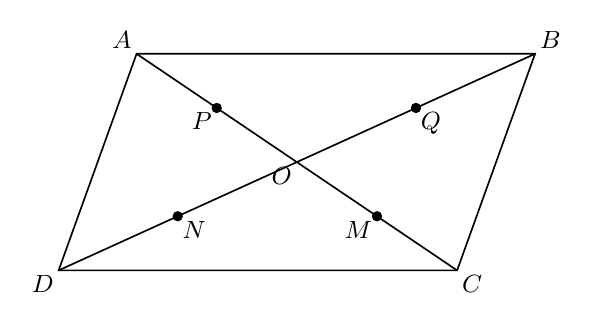
\begin{tikzpicture}[scale=1.1, semithick, every node/.style={inner sep=1.5pt, font=\small}]
  \coordinate (A) at (0.9,3.1);
  \coordinate (B) at (5.5,3.1);
  \coordinate (C) at (4.6,0.6);
  \coordinate (D) at (0,0.6);
  \coordinate (O) at (2.75,1.85);
  \coordinate (P) at (1.825,2.475);
  \coordinate (Q) at (4.125,2.475);
  \coordinate (M) at (3.675,1.225);
  \coordinate (N) at (1.375,1.225);

  \draw (A) -- (B) -- (C) -- (D) -- cycle;
  \draw (A) -- (C);
  \draw (B) -- (D);

  \fill (P) circle (1.7pt);
  \fill (Q) circle (1.7pt);
  \fill (M) circle (1.7pt);
  \fill (N) circle (1.7pt);

  \node[above left] at (A) {$A$};
  \node[above right] at (B) {$B$};
  \node[below right] at (C) {$C$};
  \node[below left] at (D) {$D$};
  \node[below left] at (O) {$O$};
  \node[below left] at (P) {$P$};
  \node[below right] at (Q) {$Q$};
  \node[below left] at (M) {$M$};
  \node[below right] at (N) {$N$};
\end{tikzpicture}
\end{center}
\nopagebreak[4]
\Needspace{4\baselineskip}
\textbf{解析}
\Needspace{5\baselineskip}
以 $O$ 为原点，$\overrightarrow{OA}=\boldsymbol a$，$\overrightarrow{OB}=\boldsymbol b$。则
\nopagebreak[4]
\[A=\boldsymbol a,\ P=\tfrac12\boldsymbol a,\ M=-\tfrac12\boldsymbol a,\ C=-\boldsymbol a;\qquad
B=\boldsymbol b,\ Q=\tfrac12\boldsymbol b,\ N=-\tfrac12\boldsymbol b,\ D=-\boldsymbol b.\]
\Needspace{5\baselineskip}
故 $\overrightarrow{OG}=\overrightarrow{OE}+\overrightarrow{OF}=s\boldsymbol a+t\boldsymbol b$，其中
\nopagebreak[4]
\[s,t\in\left\{1,\ \tfrac12,\ -\tfrac12,\ -1\right\}.\]
平行四边形 $ABCD$ 的四个顶点在 $(\boldsymbol a,\boldsymbol b)$ 坐标下为 $(1,0)$、$(0,1)$、$(-1,0)$、$(0,-1)$，即区域 $|s|+|t|\leqslant1$。
\Needspace{5\baselineskip}
$4\times4=16$ 种 $(E,F)$ 等可能，其中 $|s|+|t|\leqslant1$ 的情形只有 $|s|=|t|=\dfrac12$，共 $4$ 种，这 $4$ 个点落在边界上；其余 $12$ 个点满足 $|s|+|t|>1$，落在平行四边形外。故所求概率为
\nopagebreak[4]
\[\frac{12}{16}=\frac34.\]

\gkanswer{答案：$\dfrac34$。}

\end{answer}
\begin{answer}
\gksolhead{18}{}

\textbf{题目}：

在 $\triangle ABC$ 中，角 $A$，$B$，$C$ 所对的边分别为 $a$，$b$，$c$。设 $S$ 为 $\triangle ABC$ 的面积，满足 $S=\dfrac{\sqrt3}{4}(a^2+b^2-c^2)$。

（1）求角 $C$ 的大小；

（2）求 $\sin A+\sin B$ 的最大值。

\Needspace{4\baselineskip}
\textbf{解析}
\Needspace{5\baselineskip}
（1）由面积公式 $S=\dfrac12ab\sin C$ 与余弦定理 $a^2+b^2-c^2=2ab\cos C$，题设 $S=\dfrac{\sqrt3}4(a^2+b^2-c^2)$ 化为
\nopagebreak[4]
\[\frac12ab\sin C=\frac{\sqrt3}4\cdot2ab\cos C\iff\sin C=\sqrt3\cos C.\]
因 $C\in(0,\pi)$，$\sin C>0$，故 $\cos C>0$，$\tan C=\sqrt3$，得 $C=\dfrac\pi3$。
\Needspace{5\baselineskip}
（2）$A+B=\pi-C=\dfrac{2\pi}3$，由和差化积
\nopagebreak[4]
\[\sin A+\sin B=2\sin\frac{A+B}2\cos\frac{A-B}2
=2\sin\frac\pi3\cos\frac{A-B}2=\sqrt3\cos\frac{A-B}2\leqslant\sqrt3,\]
等号在 $\dfrac{A-B}2=0$ 即 $A=B=\dfrac\pi3$ 时成立。故最大值为 $\sqrt3$。

\gkanswer{答案：（1）$\dfrac{\pi}{3}$；（2）$\sqrt3$。}

\end{answer}
\begin{answer}
\gksolhead{19}{}

\textbf{题目}：

设 $a_1$，$d$ 为实数，首项为 $a_1$，公差为 $d$ 的等差数列 $\{a_n\}$ 的前 $n$ 项和为 $S_n$，满足 $S_5S_6+15=0$。

（1）若 $S_5=5$，求 $S_6$ 及 $a_1$；

（2）求 $d$ 的取值范围。

\Needspace{4\baselineskip}
\textbf{解析}
\Needspace{5\baselineskip}
由等差数列求和公式
\nopagebreak[4]
\[S_n=na_1+\frac{n(n-1)}2d.\]
\Needspace{5\baselineskip}
（1）由 $S_5S_6+15=0$ 与 $S_5=5$ 得 $5S_6=-15$，$S_6=-3$。于是
\nopagebreak[4]
\[a_6=S_6-S_5=-8.\]
又 $S_5=5a_1+10d=5$，即 $a_1+2d=1$；而 $a_6=a_1+5d=-8$。相减得 $3d=-9$，$d=-3$，回代得 $a_1=7$。
\Needspace{5\baselineskip}
（2）$S_5=5a_1+10d$，$S_6=6a_1+15d$，故
\nopagebreak[4]
\[(5a_1+10d)(6a_1+15d)=-15,\]
\Needspace{5\baselineskip}
展开并除以 $15$：
\nopagebreak[4]
\[2a_1^2+9a_1d+10d^2+1=0.\]
\Needspace{5\baselineskip}
对任意实数 $d$，这是关于 $a_1$ 的实系数二次方程，须有实根，故判别式非负：
\nopagebreak[4]
\[\Delta=81d^2-8\left(10d^2+1\right)=d^2-8\geqslant0,\]
\Needspace{5\baselineskip}
即 $d\leqslant-2\sqrt2$ 或 $d\geqslant2\sqrt2$。反之 $d^2\geqslant8$ 时 $\Delta\geqslant0$，取 $a_1=\dfrac{-9d\pm\sqrt{d^2-8}}4$ 即满足条件。故
\nopagebreak[4]
\[d\in(-\infty,-2\sqrt2]\cup[2\sqrt2,+\infty).\]

\gkanswer{答案：（1）$S_6=-3$，$a_1=7$；（2）$(-\infty,-2\sqrt2]\cup[2\sqrt2,+\infty)$。}

\end{answer}
\begin{answer}
\gksolhead{20}{}

\textbf{题目}：

如图，在平行四边形 $ABCD$ 中，$AB=2BC$，$\angle ABC=120^\circ$。$E$ 为线段 $AB$ 的中点，将 $\triangle ADE$ 沿直线 $DE$ 翻折成 $\triangle A'DE$，使平面 $A'DE\perp$ 平面 $BCD$，$F$ 为线段 $A'C$ 的中点。

（1）求证：$BF\parallel$ 平面 $A'DE$；

（2）设 $M$ 为线段 $DE$ 的中点，求直线 $FM$ 与平面 $A'DE$ 所成角的余弦值。
\nopagebreak[4]
\begin{center}% 2010 年浙江卷文科第 20 题：平行四边形 ABCD 沿 DE 翻折成 △A'DE（透视示意）。
% 来源 PDF：普通高考/2010/2010浙江文.pdf，SHA-256 a73e22ea405697775b2d5cd82532fcffad0f506b849d9f199265b4297b8a754b。
% 原页：第 2 页（A3 三栏）第 1 栏下部，书页码 642。
% 重绘依据：照原页透视，A 左下、E 在 AB 中点、B 右下、D 左、C 右、A' 在上；
%   F 为 A'C 中点、M 为 DE 中点。原页虚线为 D–C 与 M–F，其余（AE、EB、AD、DE、
%   A'D、A'E、A'C、BC、BF）均为实线。
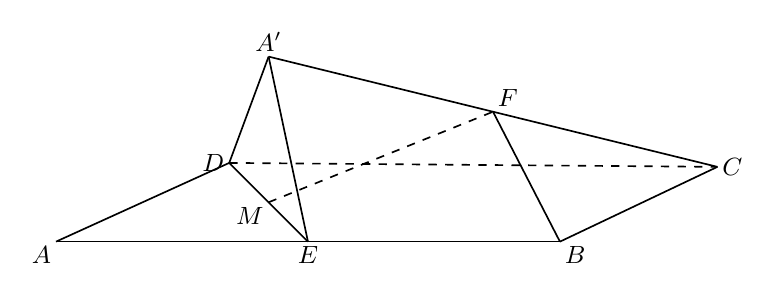
\begin{tikzpicture}[scale=1.0, semithick, every node/.style={inner sep=1.5pt, font=\small}]
  \coordinate (A)  at (0,0);
  \coordinate (E)  at (3.2,0);
  \coordinate (B)  at (6.4,0);
  \coordinate (D)  at (2.2,1.0);
  \coordinate (C)  at (8.4,0.95);
  \coordinate (Ap) at (2.7,2.35);
  \coordinate (F)  at (5.55,1.65);
  \coordinate (M)  at (2.7,0.5);

  % 底面与侧面
  \draw (A) -- (E) -- (B);
  \draw (A) -- (D);
  \draw (D) -- (E);
  \draw (B) -- (C);

  % 翻折后的三角形
  \draw (Ap) -- (D);
  \draw (Ap) -- (E);
  \draw (Ap) -- (C);
  \draw (B) -- (F);

  % 虚线：被遮挡的 D–C 与线段 M–F
  \draw[dashed] (D) -- (C);
  \draw[dashed] (M) -- (F);

  \node[above] at (Ap) {$A'$};
  \node[above right] at (F) {$F$};
  \node[below left] at (A) {$A$};
  \node[below] at (E) {$E$};
  \node[below right] at (B) {$B$};
  \node[left] at (D) {$D$};
  \node[right] at (C) {$C$};
  \node[below left] at (M) {$M$};
\end{tikzpicture}
\end{center}
\nopagebreak[4]
\Needspace{4\baselineskip}
\textbf{解析}
\Needspace{5\baselineskip}
不妨设 $BC=AD=2$，则 $AB=4$，$E$ 为 $AB$ 中点给 $AE=2$。以 $A$ 为原点、$AB$ 为 $x$ 轴、平面 $BCD$ 为 $z=0$ 建系。由 $\angle DAB=180^\circ-\angle ABC=60^\circ$，$AD=2$：
\nopagebreak[4]
\[A(0,0,0),\ B(4,0,0),\ D(1,\sqrt3,0),\ C(5,\sqrt3,0),\ E(2,0,0).\]
此时 $AE=AD=DE=2$，$\triangle ADE$ 为正三角形，$M\left(\dfrac32,\dfrac{\sqrt3}2,0\right)$ 为 $DE$ 中点，且 $AM\perp DE$，$AM=\sqrt3$。
\Needspace{5\baselineskip}
平面 $A'DE\perp$ 平面 $BCD$，故 $A'$ 在过 $M$ 且垂直于底面的直线上，$A'M=\sqrt3$：
\nopagebreak[4]
\[A'\left(\frac32,\frac{\sqrt3}2,\sqrt3\right).\]
\Needspace{5\baselineskip}
（1）$F$ 为 $A'C$ 中点：
\nopagebreak[4]
\[F\left(\frac{\frac32+5}2,\frac{\frac{\sqrt3}2+\sqrt3}2,\frac{\sqrt3}2\right)
=\left(\frac{13}4,\frac{3\sqrt3}4,\frac{\sqrt3}2\right).\]
\Needspace{5\baselineskip}
平面 $A'DE$ 的法向量
\nopagebreak[4]
\[\boldsymbol n=\overrightarrow{DE}\times\overrightarrow{DA'}
=(1,-\sqrt3,0)\times\left(\tfrac12,-\tfrac{\sqrt3}2,\sqrt3\right)=(-3,-\sqrt3,0).\]
\Needspace{5\baselineskip}
而
\nopagebreak[4]
\[\overrightarrow{BF}=\left(\frac{13}4-4,\frac{3\sqrt3}4,\frac{\sqrt3}2\right)
=\left(-\frac34,\frac{3\sqrt3}4,\frac{\sqrt3}2\right),\]
\nopagebreak[4]
\[\overrightarrow{BF}\cdot\boldsymbol n=\frac94-\frac94+0=0.\]
又 $\overrightarrow{BD}=(-3,\sqrt3,0)$，$\overrightarrow{BD}\cdot\boldsymbol n=9-3=6\neq0$，即 $B$ 不在平面 $A'DE$ 内。故 $BF\parallel$ 平面 $A'DE$。
\Needspace{5\baselineskip}
（2）
\nopagebreak[4]
\[\overrightarrow{FM}=\left(\frac32-\frac{13}4,\frac{\sqrt3}2-\frac{3\sqrt3}4,-\frac{\sqrt3}2\right)
=\left(-\frac74,-\frac{\sqrt3}4,-\frac{\sqrt3}2\right),\]
\nopagebreak[4]
\[|FM|=\sqrt{\frac{49}{16}+\frac3{16}+\frac{12}{16}}=2,\qquad
|\boldsymbol n|=\sqrt{9+3}=2\sqrt3.\]
\Needspace{5\baselineskip}
设直线 $FM$ 与平面 $A'DE$ 所成角为 $\theta$，则
\nopagebreak[4]
\[\sin\theta=\frac{|\overrightarrow{FM}\cdot\boldsymbol n|}{|FM|\cdot|\boldsymbol n|}
=\frac{\left|\frac{21}4+\frac34\right|}{2\cdot2\sqrt3}=\frac6{4\sqrt3}=\frac{\sqrt3}2,\]
故 $\theta=60^\circ$，$\cos\theta=\dfrac12$。

\gkanswer{答案：（1）证明；（2）$\dfrac12$。}

\end{answer}
\begin{answer}
\gksolhead{21}{}

\textbf{题目}：

已知函数 $f(x)=(x-a)^2(x-b)$（$a$，$b\in\mathbf R$，$a<b$）。

（1）当 $a=1$，$b=2$ 时，求曲线 $y=f(x)$ 在点 $(2,f(2))$ 处的切线方程；

（2）设 $x_1$，$x_2$ 是 $f(x)$ 的两个极值点，$x_3$ 是 $f(x)$ 的一个零点，且 $x_3\neq x_1$，$x_3\neq x_2$。证明：存在实数 $x_4$，使得 $x_1$，$x_2$，$x_3$，$x_4$ 按某种顺序排列后成等差数列，并求 $x_4$。

\Needspace{4\baselineskip}
\textbf{解析}
\Needspace{5\baselineskip}
（1）$a=1$，$b=2$ 时 $f(x)=(x-1)^2(x-2)$，
\nopagebreak[4]
\[f'(x)=2(x-1)(x-2)+(x-1)^2=(x-1)(3x-5).\]
$f(2)=0$，$f'(2)=1$，故切线为 $y=1\cdot(x-2)$，即 $x-y-2=0$。
\Needspace{5\baselineskip}
（2）一般地
\nopagebreak[4]
\[f'(x)=2(x-a)(x-b)+(x-a)^2=(x-a)\left(3x-a-2b\right).\]
两根为 $x_1=a$ 与 $x_2=\dfrac{a+2b}3$，且由 $a<b$ 得 $a<\dfrac{a+2b}3<b$。$f$ 的零点为 $a$（二重）与 $b$；因 $x_3\neq x_1=a$ 且 $x_3\neq x_2$，故 $x_3=b$。
设 $x_1,x_2,x_3,x_4$ 的某种排列为 $p,p+d,p+2d,p+3d$（$d\neq0$）。三个已知数 $a<\dfrac{a+2b}3<b$ 必占据四个位置中的三个：
\begin{itemize}
\item 若占第 $1,2,3$ 位或第 $2,3,4$ 位，则中间项同时等于 $\dfrac{a+2b}3$ 与 $\dfrac{a+b}2$，得 $a=b$，矛盾；
\item 若占第 $1,2,4$ 位，则 $3\left(\dfrac{a+2b}3-a\right)=b-a$，得 $\dfrac{a+2b}3=\dfrac{2a+b}3$，仍得 $a=b$，矛盾；
\item 只能占第 $1,3,4$ 位：此时
\end{itemize}
\nopagebreak[4]
\[\frac{a+2b}3-a=2d,\qquad b-\frac{a+2b}3=d\Rightarrow d=\frac{b-a}3,\]
缺的第 $2$ 项为 $a+d=\dfrac{2a+b}3$。
\Needspace{5\baselineskip}
取 $x_4=\dfrac{2a+b}3$，则 $a<x_4<\dfrac{a+2b}3<b$，且
\nopagebreak[4]
\[x_4-a=\frac{b-a}3,\quad \frac{a+2b}3-x_4=\frac{b-a}3,\quad b-\frac{a+2b}3=\frac{b-a}3,\]
即 $a,x_4,x_2,b$ 依次成公差为 $\dfrac{b-a}3$ 的等差数列（排列 $x_1,x_4,x_2,x_3$）。故这样的 $x_4$ 存在且唯一，$x_4=\dfrac{2a+b}3$。

\gkanswer{答案：（1）$x-y-2=0$；（2）$x_4=\dfrac{2a+b}{3}$。}

\end{answer}
\begin{answer}
\gksolhead{22}{}

\textbf{题目}：

已知 $m$ 是非零实数，抛物线 $C:y^2=2px$（$p>0$）的焦点 $F$ 在直线 $l:x-my-\dfrac{m^2}{2}=0$ 上。

（1）若 $m=2$，求抛物线 $C$ 的方程；

（2）设直线 $l$ 与抛物线 $C$ 交于 $A$，$B$ 两点，过 $A$，$B$ 分别作抛物线 $C$ 的准线的垂线，垂足为 $A_1$，$B_1$，$\triangle AA_1F$，$\triangle BB_1F$ 的重心分别为 $G$，$H$。求证：对任意非零实数 $m$，抛物线 $C$ 的准线与 $x$ 轴的交点在以线段 $GH$ 为直径的圆外。
\nopagebreak[4]
\begin{center}% 2010 年浙江卷文科第 22 题：抛物线 C、准线、焦点 F，以及 △AA_1F、△BB_1F 的重心 G、H。
% 来源 PDF：普通高考/2010/2010浙江文.pdf，SHA-256 a73e22ea405697775b2d5cd82532fcffad0f506b849d9f199265b4297b8a754b。
% 原页：第 2 页（A3 三栏）第 3 栏上部，书页码 642。
% 重绘依据：照原页，抛物线开口向右、顶点在原点 O；准线为左侧竖直线，
%   A_1、B_1 在准线上且 A_1A、B_1B 水平；弦 AB 过焦点 F（即直线 l）；
%   连 A_1F、B_1F，标出重心 G、H（原页无圆，只标两点）。
%   题设 p=m^2，取 m=0.35（p=0.1225）并按 p/2 归一化作图，得 y^2=4x、准线 x=-1、
%   F(1,0)、A(1.99,2.82)、B(0.50,-1.42)、G(0.66,1.88)、H(0.17,-0.95)。
\begin{tikzpicture}[scale=1.05, semithick, every node/.style={inner sep=1.2pt, font=\small}]

  % 抛物线 y^2 = 4x，即 x = y^2/4
  \draw[domain=-1.55:3.0, samples=160, smooth, variable=\y]
    plot ({(\y*\y)/4}, \y);

  % 坐标轴
  \draw[->, >=stealth] (-1.3,0) -- (3.9,0);
  \draw[->, >=stealth] (0,-1.6) -- (0,3.05);
  \node[below right] at (3.9,0) {$x$};
  \node[left] at (0,3.05) {$y$};

  % 准线
  \draw (-1,-1.5) -- (-1,2.95);

  % 关键点
  \coordinate (A1) at (-1,2.82);
  \coordinate (B1) at (-1,-1.42);
  \coordinate (A)  at (1.99,2.82);
  \coordinate (B)  at (0.50,-1.42);
  \coordinate (F)  at (1,0);
  \coordinate (G)  at (0.663,1.88);
  \coordinate (H)  at (0.167,-0.947);

  % 水平投影线与连线
  \draw (A1) -- (A);
  \draw (B1) -- (B);
  \draw (A1) -- (F);
  \draw (B1) -- (F);
  \draw (A) -- (B);

  \fill (G) circle (1.7pt);
  \fill (H) circle (1.7pt);

  \node[left] at (A1) {$A_1$};
  \node[left] at (B1) {$B_1$};
  \node[above left] at (A) {$A$};
  \node[below right] at (B) {$B$};
  \node[below right] at (F) {$F$};
  \node[below left] at (0,0) {$O$};
  \node[left] at (G) {$G$};
  \node[right] at ($(H)+(0.06,0.09)$) {$H$};
\end{tikzpicture}
\end{center}
\nopagebreak[4]
\Needspace{4\baselineskip}
\textbf{解析}
\Needspace{5\baselineskip}
（1）焦点 $F\left(\dfrac p2,0\right)$ 在 $l:x-my-\dfrac{m^2}2=0$ 上，故
\nopagebreak[4]
\[\frac p2-\frac{m^2}2=0\Rightarrow p=m^2.\]
当 $m=2$ 时 $p=4$，$C:y^2=8x$。
\Needspace{5\baselineskip}
（2）此时 $p=m^2$，$l:x-my-\dfrac p2=0$ 恰过焦点 $F\left(\dfrac p2,0\right)$。代入 $y^2=2px$：
\nopagebreak[4]
\[y^2=2p\left(my+\frac p2\right)\Rightarrow y^2-2pmy-p^2=0,\]
\Needspace{5\baselineskip}
故
\nopagebreak[4]
\[y_1+y_2=2pm,\qquad y_1y_2=-p^2.\]
\Needspace{5\baselineskip}
由 $x_i=\dfrac{y_i^2}{2p}$ 得
\nopagebreak[4]
\[x_1+x_2=\frac{(y_1+y_2)^2-2y_1y_2}{2p}=\frac{4p^2m^2+2p^2}{2p}=p(2m^2+1),\]
\nopagebreak[4]
\[x_1x_2=\frac{(y_1y_2)^2}{4p^2}=\frac{p^2}4.\]
\Needspace{5\baselineskip}
准线 $x=-\dfrac p2$ 与 $x$ 轴交于 $D\left(-\dfrac p2,0\right)$，且 $A_1\left(-\dfrac p2,y_1\right)$，$B_1\left(-\dfrac p2,y_2\right)$。$\triangle AA_1F$ 的重心
\nopagebreak[4]
\[G\left(\frac{x_1-\frac p2+\frac p2}3,\frac{y_1+y_1+0}3\right)=\left(\frac{x_1}3,\frac{2y_1}3\right),\]
\Needspace{5\baselineskip}
同理 $H\left(\dfrac{x_2}3,\dfrac{2y_2}3\right)$。点 $D$ 在以 $GH$ 为直径的圆外，等价于 $\angle GDH$ 为锐角，即
\nopagebreak[4]
\[\overrightarrow{DG}\cdot\overrightarrow{DH}>0.\]
\Needspace{5\baselineskip}
计算
\nopagebreak[4]
\[\overrightarrow{DG}\cdot\overrightarrow{DH}
=\left(\frac p2+\frac{x_1}3\right)\left(\frac p2+\frac{x_2}3\right)+\frac49y_1y_2\]
\nopagebreak[4]
\[=\frac{p^2}4+\frac p6(x_1+x_2)+\frac{x_1x_2}9+\frac49y_1y_2
=\frac{p^2}4+\frac{p^2(2m^2+1)}6+\frac{p^2}{36}-\frac{4p^2}9=\frac{p^2m^2}3>0,\]
因 $p>0$，$m\neq0$，故对任意非零实数 $m$，$D$ 恒在以 $GH$ 为直径的圆外。

\gkanswer{答案：（1）$y^2=8x$；（2）证明。}

\end{answer}